% !TeX spellcheck = ru_RU
\documentclass{beamer}
\setbeamertemplate{navigation symbols}{}


\usetheme{Frankfurt}

\usepackage{amsmath,amssymb,amsthm,amscd,amsfonts, mathtools}
\usepackage[utf8]{inputenc}
\usepackage[english, russian]{babel}
\usepackage{wrapfig}

\makeatletter
\newcommand*{\rom}[1]{\expandafter\@slowromancap\romannumeral #1@}
\newcommand\setItemnumber[1]{\setcounter{enum\romannumeral\@enumdepth}{\numexpr#1-1\relax}}
\makeatother

\newtheorem{definition_}{Определение}
\newtheorem{target_}{Цель работы}
\newtheorem{prob_task}{Вероятностная постановка задачи классификации}
\newtheorem{algo_task}{Алгоритмическая постановка задачи классификации}
\newtheorem{prob_def}{Вероятностное определение $w_{ij}^k$}
\newtheorem{algo_def}{Алгоритмическое определение $w_{ij}^k$}

\begin{document}
	\title{Синолитические сети в классификации мозговой активности}  
	\author{Власенко Даниил\\
	{\footnotesize Научные руководители: Заикин Алесей, Захаров Денис Геннадьевич}
%	{\footnotesize Научные руководитель: Шпилёв Пётр Валерьевич}
	}
	\date{\today} 
	
	\begin{frame}
		\titlepage
	\end{frame}

	\begin{frame}
		\frametitle{Содержание}
		\tableofcontents
	\end{frame} 

	\section{Введение} 
	\begin{frame}
		\frametitle{фМРТ} 
							
		\begin{definition_}
			Функциональная магнитно-резонансная томография или фМРТ~--- разновидность магнитно-резонансной томографии, которая проводится с целью измерения изменений в токе крови, вызванных нейронной активностью головного или спинного мозга. 
		\end{definition_}
	
		\begin{figure}
			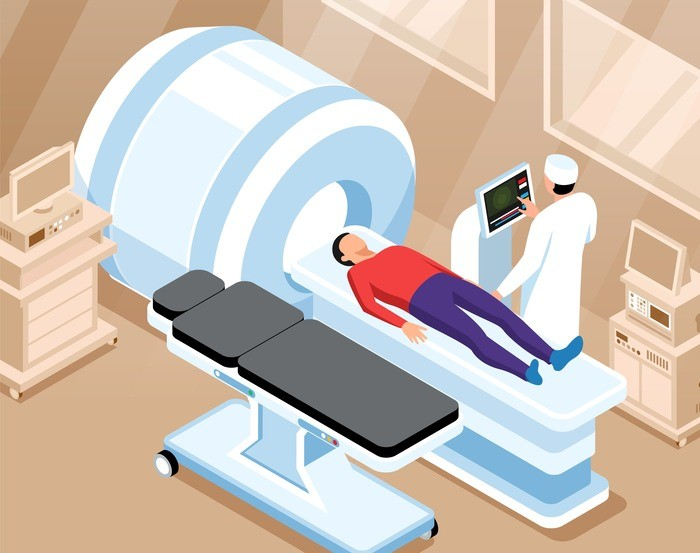
\includegraphics[width=4cm]{../images/fmri_1.jpeg}
			\caption{фМРТ сканер.} 
			\label{fg:1}
		\end{figure}		
	\end{frame}

	\begin{frame} 
		\frametitle{фМРТ}
		\begin{figure}
			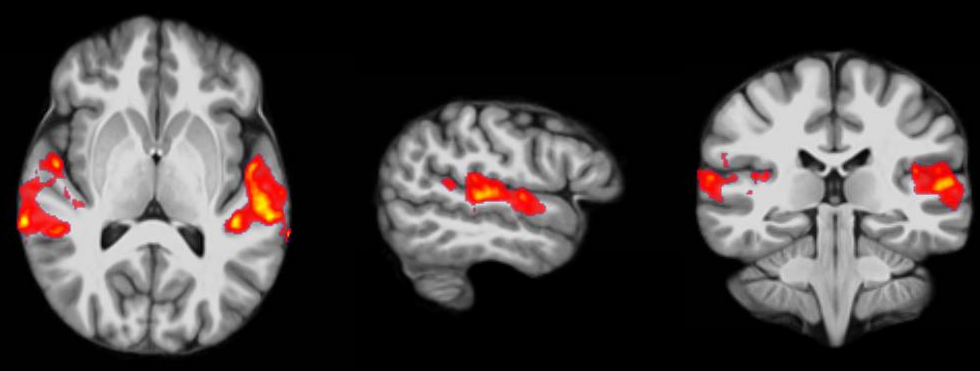
\includegraphics[width=10cm]{../images/fmri_2.png}
			\caption{МРТ скан.} 
			\label{fg:2}
		\end{figure}
	\end{frame}

	\begin{frame} 
		\frametitle{Цель работы}
		Будем считать, что мозг может функционировать в двух режимах.
		
		\begin{target_}
			Реализация и тестирование нового метода классификации режимов мозговой активности на основе фМРТ данных.
		\end{target_}			
	\end{frame}

	\begin{frame} 
		\frametitle{Классификация}
		\begin{prob_task}
			Пусть есть с.в. $\xi: \Omega \rightarrow X$ и с.в. $\eta: \Omega \rightarrow Y$. Рассмотрим с.в. $(\xi, \eta): \Omega \rightarrow (X, Y)$ с распределением $p(x, y)$.
			\vspace{0.5cm}
			
			Задача классификации сводится оценке $p(y|x)$ по выборке $(\widetilde{X}, \widetilde{Y}) = \{(x_{k}, y_{k}), k = 1, \dots, N\}$
		\end{prob_task}
	
		\begin{algo_task}
			Пусть $X$ --- множество описаний объектов, $Y$ --- множество номеров классов. Существует функция $f: X \rightarrow Y$, значения которой известны только на объектах выборки $(\widetilde{X}, \widetilde{Y}) =  \{(x_{k}, y_{k}), k = 1, \dots, N\}$. 
			\vspace{0.5cm}
			
			Требуется построить алгоритм-оценку $\widehat{f}: X \rightarrow Y$.
		\end{algo_task}
	\end{frame}

	\begin{frame} 	
		\frametitle{Векторизация}	
		
		NiBabel --- библиотека предоставляющая возможность читать различные форматы файлов нейровизуализации.
		\vspace{0.5cm}
				
		\begin{figure}
			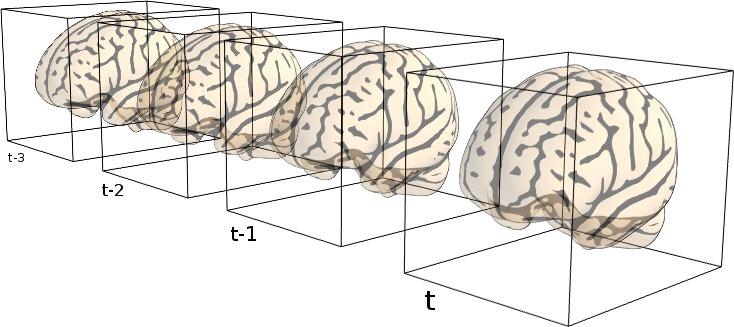
\includegraphics[width=7cm]{../images/vectorization_1.png}
			\caption{Векторизация фМРТ данных.} 
			\label{fg:5}
		\end{figure}
	\end{frame}
	
	\section{Синолитические сети}
	\begin{frame} 
		\frametitle{Основная идея (Zaikin Alexey 2022)}
		\begin{figure}
			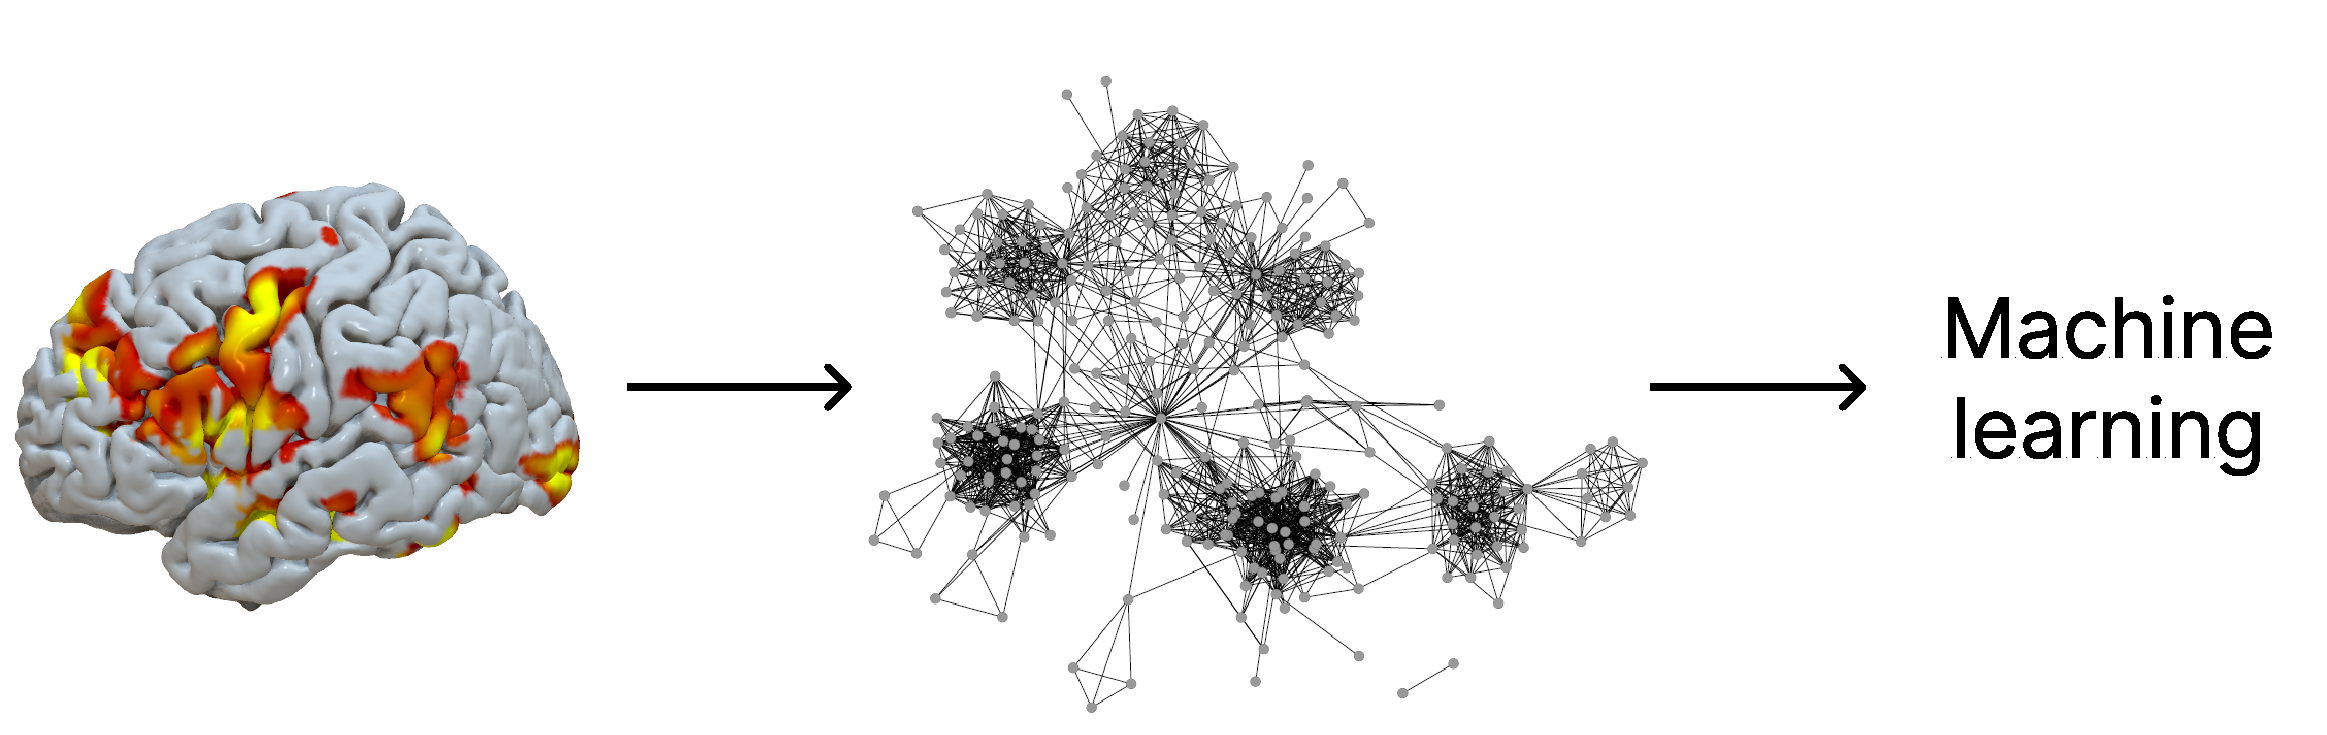
\includegraphics[width=10cm]{../images/fmri_graph_ml_1.pdf}
			\caption{Классификация на основе построения графов отражающих входные данные.} 
			\label{fg:3}
		\end{figure}
	\end{frame}

	\begin{frame} 
		\frametitle{Обозначения}
		Пусть $X = \{x_k\}_k$ --- множество фМРТ, а $Y = \{y_k\}_k$ --- режимы когнитивной активности $\{x_k\}_k$ со значениями $\rom{1}$ или  $\rom{2}$.
		\vspace{0.5cm}
		
		$x_k \in X$ конвертируется в массив $a^k$, на основе которого строиться граф $g_k = (V_k, E_k, R_k, W_k)$, где 
		\begin{itemize}
			\item $V_k = \{v_i^k\}_i$ --- множество вершин,
			\item $E_k = \{e_{ij}^k\}_{ij}$ --- множество неориентированных ребер,
			\item $R_k = \{r_i^k\}_i$ --- множество значений вершин,
			\item $W_k = \{w_{ij}^k\}_{ij}$ --- множество весов ребер,
			\item $v_i^k$ --- вершина отражающая область мозга $i$,
			\item $e_{ij}^k$ --- ребро отражающее связь между областями $i$ и $j$,
			\item $r_i^k$ -- значение вершины $v_i^k$,
			\item $w_{ij}^k$ -- вес ребра $e_{ij}^k$.
		\end{itemize}									
	\end{frame}

	\begin{frame} 
		\frametitle{Подсчет весов ребер $w_{ij}^k$}						
		\begin{prob_def}
			\[
				w_{ij}^k = P(y_k = \rom{2} | r_i^k, r_j^k) - P(y_k = \rom{1} | r_i^k, r_j^k)
			\]			
		\end{prob_def}								
		Пусть $Cl_{ij}: \{y_k |(r_i^k, r_j^k), \{(r_i^n, r_j^n)\}_n, \{y_n\}_n\}_k \rightarrow [0, 1]$ --- вероятностный классификатор.
		
		\begin{algo_def}			
			\begin{equation*}
				\begin{multlined}
					w_{ij}^k = Cl_{ij}(y_k = \rom{2} | (r_i^k, r_j^k), \{(r_i^n, r_j^n)\}_n, \{y_n\}_n) - \\ - Cl_{ij}(y_k = \rom{1} | (r_i^k, r_j^k), \{(r_i^n, r_j^n)\}_n, \{y_n\}_n)
				\end{multlined}
			\end{equation*}			
		\end{algo_def}	
	\end{frame}

	\begin{frame} 
		\vspace{0.4cm}
		
		\begin{figure}
			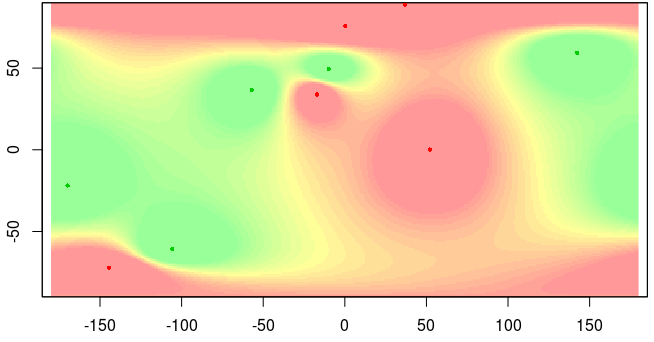
\includegraphics[width=10cm]{../images/classification.png}
			\caption{Эмпирическая плотность распределения $(r_i, r_j)$ для двух режимов, вычисленная по $\{(r_i^n, r_j^n)\}_n$} 
			\label{fg:4}
		\end{figure}
	\end{frame}	

	\section{Понижение размерности}
	\begin{frame} 
		\frametitle{Увеличение размеров вокселя}
		
		Увеличение размера шага решетки фМРТ в $n$ раз уменьшает число вокселей в $n^3$ раза.
		\vspace{0.5cm}
										
			\begin{figure}
				\begin{minipage}{3.5cm}
					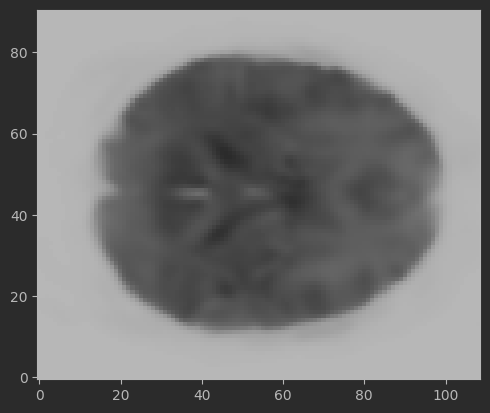
\includegraphics[width=3.5cm]{../images/downsampling2mm_1.png}
					\caption{Воксель 2 мм$^3$}
					\label{fg:6}
				\end{minipage}\hfill
				\begin{minipage}{3.5cm}
					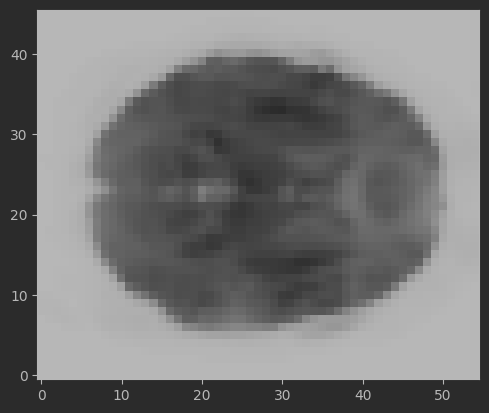
\includegraphics[width=3.5cm]{../images/downsampling4mm_2.png}
					\caption{Воксель 4 мм$^3$}
					\label{fg:7}
				\end{minipage}\hfill
				\begin{minipage}{3.5cm}
					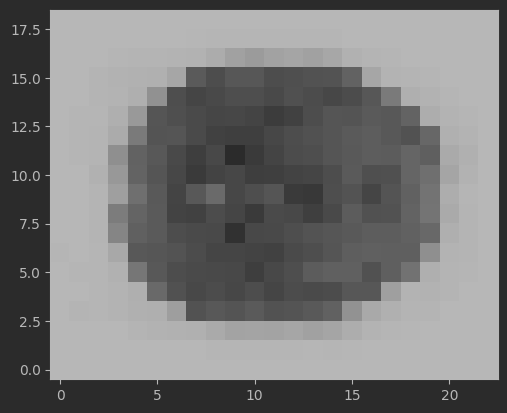
\includegraphics[width=3.5cm]{../images/downsampling10mm_3.png}
					\caption{Воксель 10 мм$^3$}
					\label{fg:8}
				\end{minipage}
			\end{figure}	
	\end{frame}
	
	\begin{frame} 
		\frametitle{Понижение размерности по времени}
		Пусть $T$ --- некоторая статистика,
		\[
		a^{kT} = T(a^k),
		\]
		т.е. для $\forall x, y, z$
		\[
		a^{kT}_{xyz} = T(\{a_{xyzt}^k : \forall t\}).
		\]
		
		\begin{figure}
			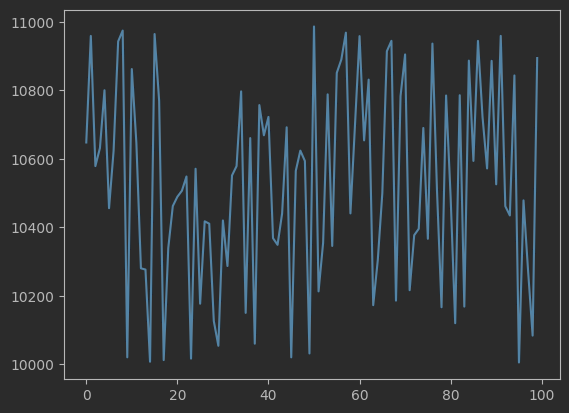
\includegraphics[width=6cm]{../images/time_series.png}
			\caption{Значения вокселя.} 
			\label{fg:11}
		\end{figure}	
	\end{frame}	

	\begin{frame} 
		\frametitle{Смена структуры графа}
		
		Переход от полного графа к графу-решетке снижает время вычисления и требуемую память с $O(n^2)$ до $O(n)$, где $n$~--- число вершин графа.
		
		\vspace{0.5cm}
						
		\begin{figure}
			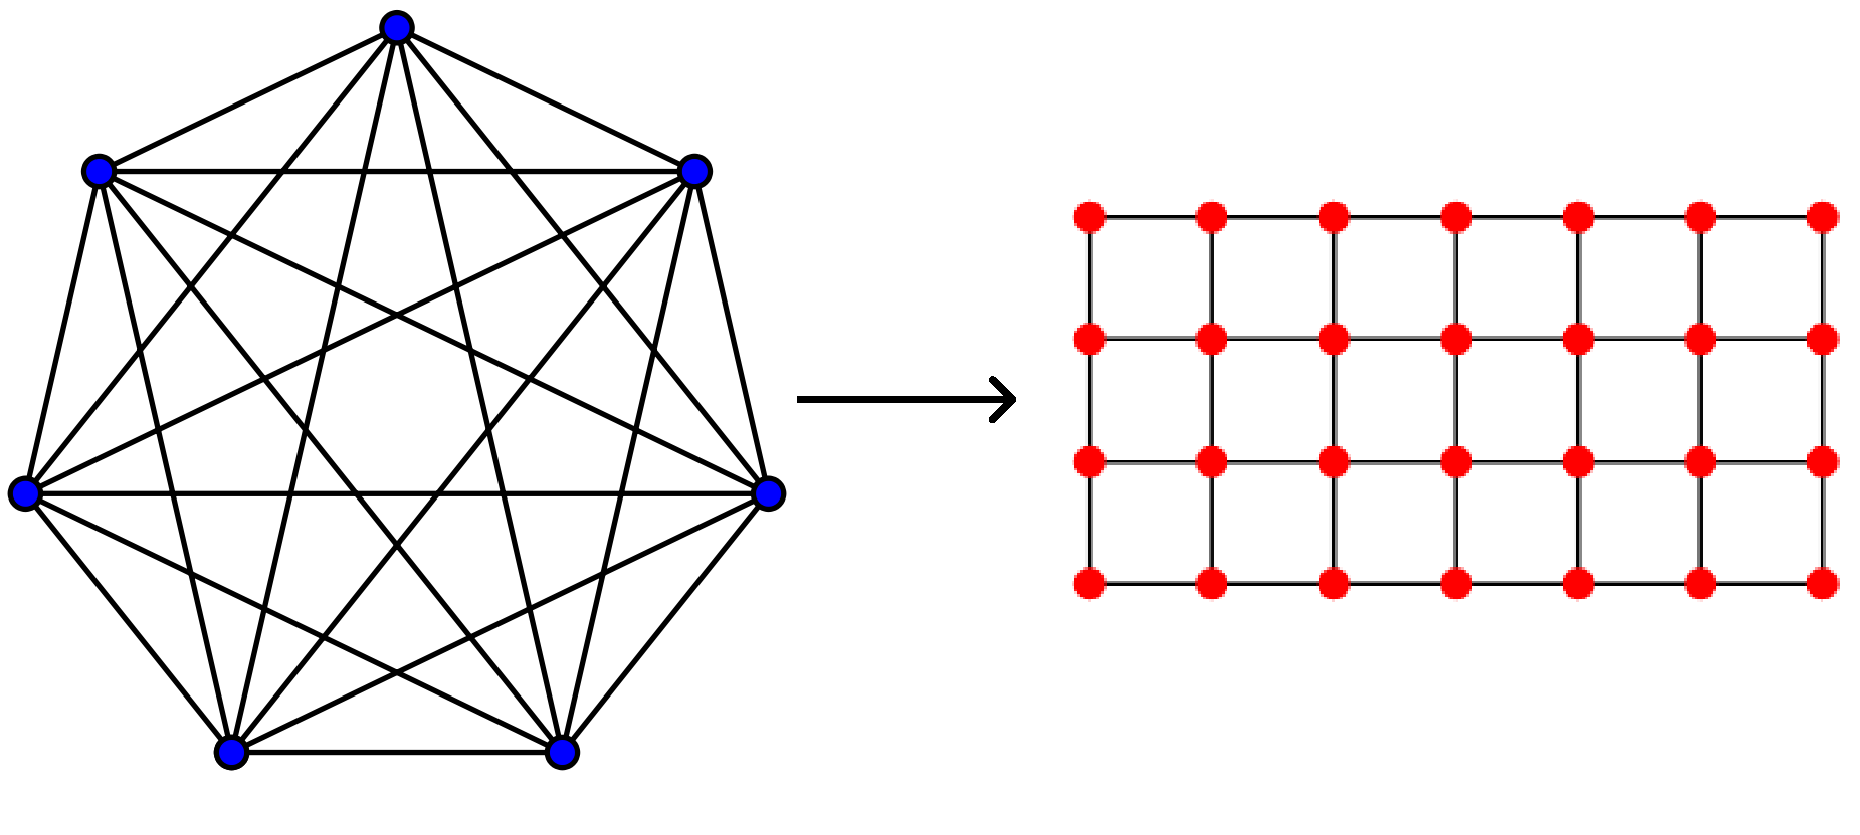
\includegraphics[width=8cm]{../images/full_grid_graphs_1.pdf}
			\caption{Переход от полного графа к графу-решетке.} 
			\label{fg:9}
		\end{figure}			
	\end{frame}	

	\section{Алгоритм}
	\begin{frame} 
		\frametitle{Обучение модели}
		Входные данные:
		\begin{itemize}
			\item выборка $(\widetilde{X}, \widetilde{Y})$,
			\item новый размер шага решетки фМРТ $s$,
			\item статистики вокселей $\{T_r\}_r$,
			\item минимальное абсолютное значение ребра $w$ для которого ребро не удаляется из графа,
			\item статистики графов $\{P_u\}_u$, на которых будет учиться модель.
		\end{itemize}
	\end{frame}

	\begin{frame} 
		\frametitle{Обучение модели}
		Алгоритм: 
		\begin{enumerate}
			\item изменение шага решетки фМРТ для $\forall x_k \in \widetilde{X}$;
			\item построение $\{a^k\}_k$;
			\item подсчет $\{a^{kT_p}\}_{kp}$;
			\item обучение  $\{Cl_{ij}\}$ на выборке $(\{a^{kT_p}\}_{kp}, \widetilde{Y})$;
			\item подсчет $W_k = \{w_{ij}^k\}_{ij}$ с помощью $\{Cl_{ij}\}_{ij}$;
			\item построение графов $g_k$ с помощью $a^{kT_p}$ и $\{w_{ij}^k\}$
		\end{enumerate}
	\end{frame}

	\section{Результаты}
	\begin{frame} 
		\frametitle{Данные}
		\begin{figure}
			\begin{minipage}{4.5cm}
				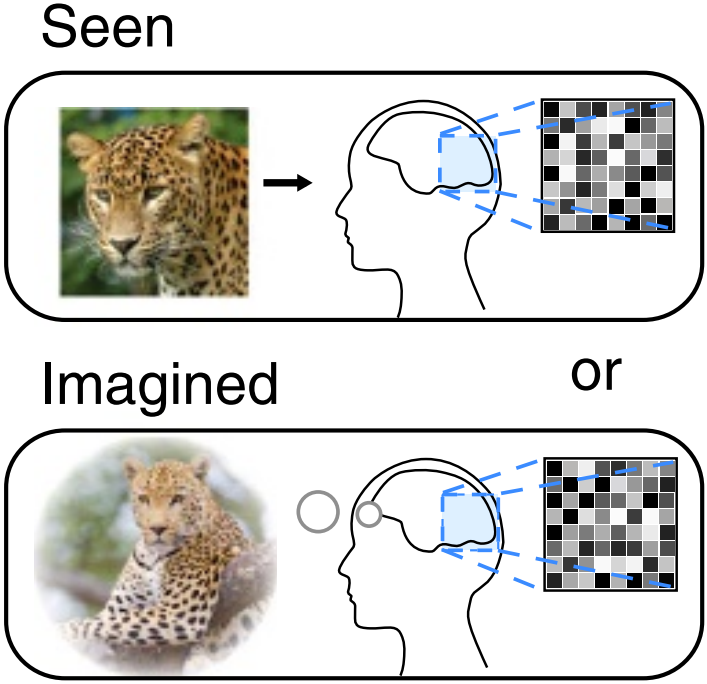
\includegraphics[width=4.5cm]{../images/data_1.png}
				\caption{Наблюдение или воображение объекта.} 
				\label{fg:12}
			\end{minipage}\hfill
			\begin{minipage}{5.5cm}
				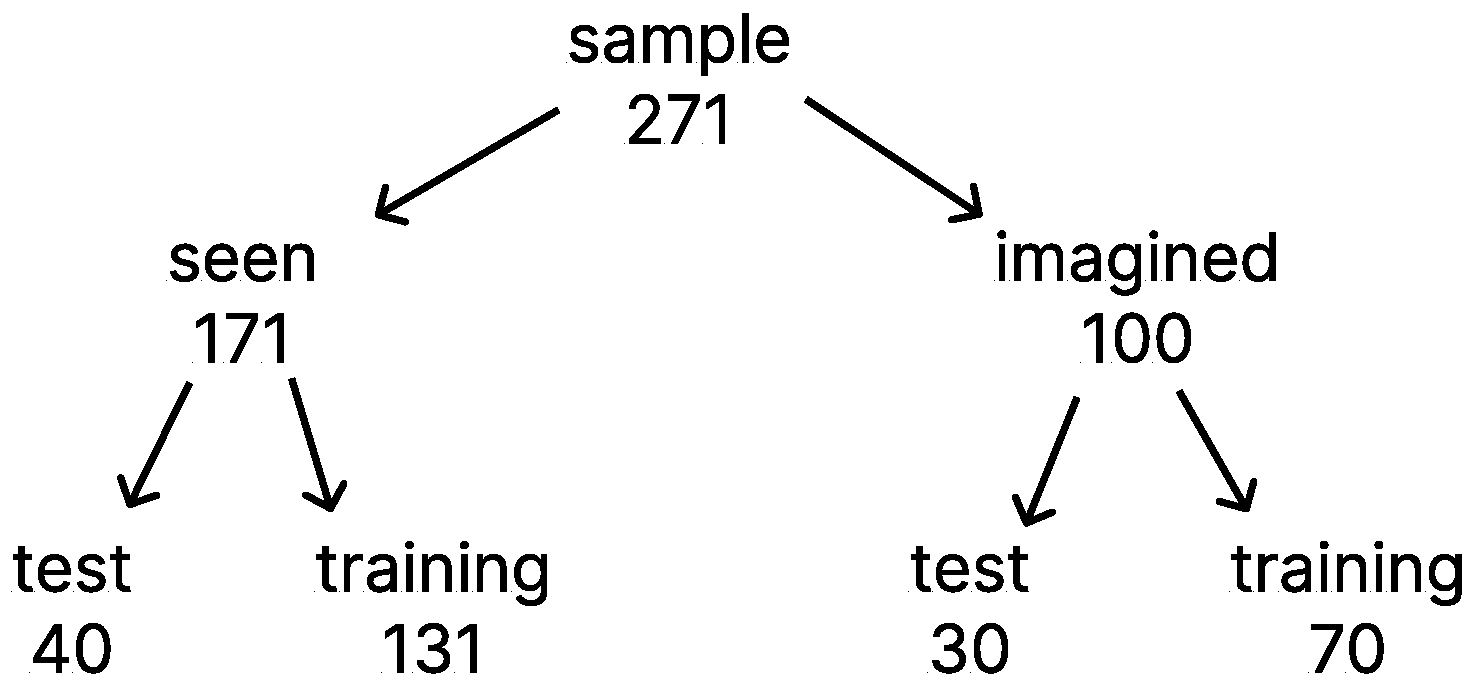
\includegraphics[width=5.5cm]{../images/data_2.pdf}
				\caption{Разделение выборки.}
				\label{fg:13}
			\end{minipage}	
		\end{figure}
	\end{frame}

	\begin{frame} 
		\frametitle{Точность классификации, \%}
		\vspace{1cm}
		
		\begin{table}
			\begin{tabular}{ccccc}
				$mean$ & $median$ & $max$ & $min$ & $max - min$ \\ \hline
				100 & 100 & 95.7 & 97.1 & 90
			\end{tabular}
		\end{table}
	
		\begin{table}
			\begin{tabular}{ccc}
				$q_{0.9}$ & $q_{0.1}$ & $q_{0.9} - q_{0.1}$ \\ \hline
				98.6 & 100 & 88.6
			\end{tabular}
		\end{table}
	
	
		

	\end{frame}
		
		


\end{document}
	